\block{Problématique}{
       { \fontsize{40}{40}\selectfont 
       
       Avec les nombreuses fuites de données récentes des entreprises et les nombreux autres problèmes de sécurité, il est important de mettre en place des mesures de sécurité robustes. Une solution à ces problèmes est d’implémenter un système biométrique. Ces systèmes permettent d'identifier une personne en utilisant des valeurs biométriques comme l’empreinte digitale, la voix, le visage ou l’iris. Les systèmes biométriques sont très sensibles et précis. En tant qu’étudiant de premier cycle, ce projet me permet d’explorer ces systèmes et de m’initier à la recherche.\cite{ref_3}
       
       }
}

\block{Objectifs}{
 	{ \fontsize{40}{40}\selectfont  
        
	\vspace{1em}
	\begin{itemize}
		\item Développer un système capable d’identifier une personne en se basant sur une image de l'iris d'un oeil en utilisant des techniques d’apprentissage automatique. 
Le système sera en mesure de prédire un résultat, afin de savoir si l'image donnée correspond à l'iris d'une personne déjà enregistrée en se basant sur les images préalablement fournies par cette même personne.
		\item Ce modèle pourra ensuite être utilisé par une application à travers
une API REST, permettant une identification par l'iris.
	\end{itemize}
        
	}
}	

\block{Description du Système}{
 	{ \fontsize{40}{40}\selectfont 
 	
	Le système construit est composé de plusieurs étapes.

    \vspace{1em}
    \begin{center}
        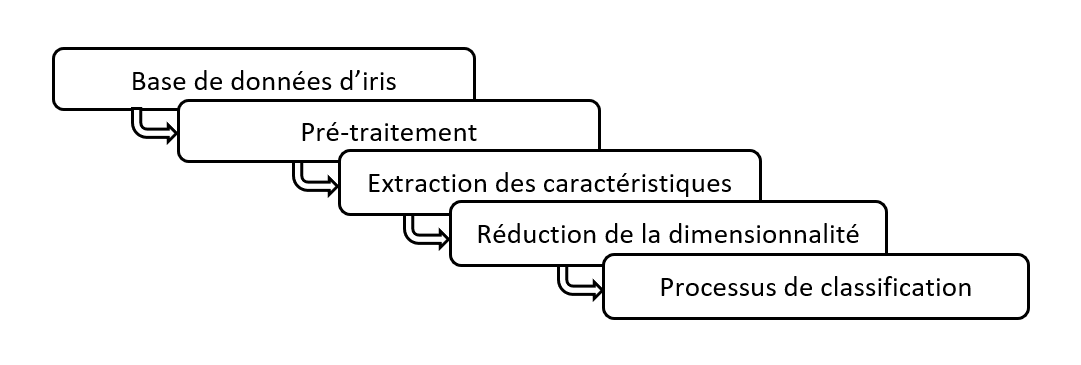
\includegraphics[width=0.9\linewidth]{schema}
        \captionof{figure}{Schéma du système.}
    \end{center}
    \vspace{1em}
    }
}